\documentclass[a4paper]{article}
\usepackage[utf8]{inputenc}
\usepackage[english]{babel}

\usepackage{amsmath}
\usepackage{amsfonts}
\usepackage{amssymb}
\usepackage{graphicx}
\usepackage{fancyhdr}
\usepackage{moreverb}
\usepackage{listings}
\usepackage{courier}
\usepackage{qtree}
\usepackage[normalem]{ulem}
\usepackage{color}
\usepackage{comment}
\usepackage{float}

\newcommand{\setR}{\mathbb{R}}
\newcommand{\setZ}{\mathbb{Z}}
\newcommand{\setN}{\mathbb{N}}
\newcommand{\setF}{\mathbb{F}}
\newcommand{\lra}{\leftrightarrow}
\newcommand{\Lra}{\Leftrightarrow}
\newcommand{\ra}{\rightarrow}
\newcommand{\Ra}{\Rightarrow}
\newcommand{\tbf}[1]{\textbf{#1}}
\newcommand{\tit}[1]{\textit{#1}}
\newcommand{\tsc}[1]{\textsc{#1}}
\newcommand{\tsf}[1]{\textsf{#1}}
\newcommand{\tsl}[1]{\textsl{#1}}
\newcommand{\ttt}[1]{\texttt{#1}}
\newcommand{\subsubsubsection}[1]{\tbf{#1}\\}
\newcommand{\makeline}[1]{\noindent\makebox[\linewidth]{\rule{#1}{0.5pt}}}


\lstset{	numbers=left,
		numberstyle=\footnotesize\ttfamily,
		numbersep=8pt,
		frame = single,
		basicstyle=\ttfamily,
		keywordstyle=\bfseries,
		commentstyle=\color{green},
		showstringspaces=false,
		morekeywords={include, printf, int, if, else, sizeof, void}
		}

\renewcommand{\headrulewidth}{0pt}

\title{Assisting Fuzzing with Concolic Execution}
\author{Søren Lund Jensen}
\begin{document}

\maketitle %TODO ændr til en flottere forside

\tableofcontents

\newpage
\section{Abstract}

\newpage
\section{Introduction and concept}
An ever-present danger in today's society is memory corruption vulnerabilities in software, be they use of uninitialized memory, using dangling null-pointers, buffer overflow, memory leaks, or a fifth, sixth- or seventh vulnerabilities. An attacker could, did he know of these vulnerabilities, exploit them in order to access confidential informations, create DOS-attacks or other and as computer processing and connecting continues to be on the rise, playing a major role in present day, patching these vulnerabilities has to be a priority. This, of course, cannot be done without first discovering said bugs. 

Memory corruption bugs are often-case virtually untraceable, as only specific input combinations may trigger them, or the fact that they may appear under very unusual conditions, which makes it very hard to discover, or in some cases, even reproduce them. Add thereto, the fact, that the memory corruption's effect may manifest itself far away from its source, it can also be hard to even correlate these two, once a bug has been discovered.

A variety of tools exists, with the purpose of bug-discovery, but as the bugs are often very specific, and/or wide-spread, creating a silver bullet is hard, if not impossible. Many vulnerabilities are discovered manually, however, this solution is not scalable, as software applications generally increase in size and complexity. A handful of tools exist, including fuzzers and symbolic execution engines. These do, however have, in the worst cases, deal-breaking flaws, working against them, and their usefulness.

In 2016, The Defence Advanced Research Projects Agency (DARPA) hosted the 2016 Cyber Grand Challenge, with the theme of promoting and advancing automated computer security techniques, ranging from bug-detection to bug-squashing to hacking - all without interference from the teams who've created the software. Among the programs, created for the competition was the Driller project: an extended version of American Fuzzy Lop, augmented by the concolic execution-engine, known as angr.

The idea behind this technology is to, through combining AFL with angr, mitigate as many of each of their respective drawbacks, while simultaneously utilizing both of their many advantages.
%TODO Måske noget med om den i virkeligheden holder.
\subsection{Problem statement}
Does Driller display a significant difference, in terms of running time and bugs/ vulnerabilities found, when compared to "regular" fuzzing, or is the technology?

Alternatively, is Driller suffering from being too narrowly engineered, as to better fit the kind of test-binaries, given by DARPA, and so, non-usable in real day, intrusion-combating?
\newpage
\section{American Fuzzy Lop}
This program works by feeding random input to a program, at a very high rate, some of which will hit specific vulnerabilities in said input-program. Every input fed is logged, and upon vulnerability-hit, AFL logs the input-ID. Hereafter information about where the vulnerability occurred, and which input triggered it is gatherable, based on input ID.

An advantage, as well as a drawback of most fuzzers, hereunder AFL is its execution method, which is to be as non-invasive as possible, as to prioritize speed before complexity handling. This means that AFL does not analyse a fuzzed application, but instead directly executing the application with random input, which is immensely faster than mutating qualified input variables, based on an application analysis.
\subsection{Features of AFL}
AFL implements a variety of features, to enhance its efficiency. In this section, I will list some of the key features, offered.\\
\subsubsubsection{Genetic Fuzzing}
When stating that the AFL fuzzing engine relies on executing applications with inputs at absolute random, one is not totally correct. This is due to the technique known as 'Genetic Fuzzing'. Genetic fuzzing means that the engine generates - \tit{unique} - inputs at total random. Simplified, this means that the current input, that AFL is generating cannot be the same as a previously generated input.  
\subsubsubsection{Stable Transition Tracking}
AFL views the union of source and destination as a tuple of it's destination blocks. These tuples are prioritised, meaning that the tuples that cause the most different execution, compared to previous executions, are chosen first for future input generation.
\subsubsubsection{Loop Bucketization}
For a symbolic execution engines and fuzzers alike, loops are complicated to handle, as looping potentially offers an added layer of complexity. The AFL fuzzer makes the following contortions, in order to avoid looping's added complexity, and path space requirements:
When AFL detects that a triggered path contains a loop, it logs the executed loop iterations and compares this with previous inputs. The paths are grouped, based on the amount of iterations, and hereafter only \tit{one} path in a group is selected for further fuzzing. Using this technique, $O(N)$ of the slow loop-including paths are executed, as opposed to $O(N)$ paths.\\
\subsubsubsection{Derandomization}
%TODO
TODO
\newpage
\subsection{Limitations of AFL}
Because of the union of the above techniques and its general nature, AFL is able to quickly discover a wide selection of general vulnerabilities, meaning vulnerabilities, that are triggered by some \tit{kind} of input. When vulnerability-triggers move past general input, and into the territory of general input AFL can potentially fall seriously behind.
\begin{lstlisting}[caption=A program that is difficult to fuzz, label=diffToFuzz, captionpos=b]
int main(void)
{
    int x;
    read(0, &x, sizeof(x));
    
    if (x == 0x12345678){
        vulnerability();
    }else{
         ...
    }
}
\end{lstlisting}
A generic example of this can be seen in Listing \ref{diffToFuzz}. This describes a program, that takes an input $x$ from a user. If, and only if, $x$ evaluates to $0x12345678$ the program will fail, as a vulnerability has been triggered, and as so, at each command, executed by the fuzzer, the frequency, and by extension, the chance of discovering the bug, is $1$ in $2^{32}$. Furthermore, as the AFL lacks the ability to produce new paths within this specific program lacks, it's instrumentation falls short, and AFL is reduced to randomly mutating non-instrumented input.
\section{Symbolic Execution}
Symbolic execution, or symbolic evaluation, is a way of program analysis, designed in order to determine the different ways said program can be executed, and which type of input causes it. Instead of executing actual values, to determine this, an interpreter assigns symbolic values to the input variables. The symbolic used to visualise how the program will execute, based on what \tit{kind} of input it will be fed.
\subsection{Features of Symbolic Execution}
As symbolic execution relies on analysing input, instead of mindlessly executing input, it is able to detect specific inputs which, in this case, cause the application to crash. See Listing \ref{diffToFuzz} as an example. A symbolic execution engine will analyse it's functions, and generate the following tree:\\
\centerline{\Tree [.$\emptyset$ [. $x==0x12345678$ $\neg(x==0x12345678)$ ] ]}
\newpage
\noindent Another advantage of symbolic execution is the ability to invalidate sections input.
\begin{lstlisting}[caption=Example of Symbolic Execution, label=SymExExample, captionpos=b]
int main(void)
{
    int y;
    read(0, &y, sizeof(y));
    
    if (y > 0x01){
        ...
    }else{
        ...
    }
    if (y > 0x10){
        ...
    }else{
        ...
    }
}
\end{lstlisting}
In Listing \ref{SymExExample} above, for example, the input $y$ is evaluated. A symbolic execution engine will analyse Listing \ref{SymExExample}'s formulae, to find that $y$ will either assume a value greater than $0x01$ or not greater than $0x01$. Furthermore $y$ will either assume a value greater, or not greater than $0x10$, however greater than $0x10$ cannot occur, if $y$, at the same time was not greater than $0x01$. This will produce the following tree:\\
\centerline{
	\Tree [.$\emptyset$
			[.$y>0x01$ 
				[. $y>10$ 
				   $\neg(y>0x10)$
				]
			]
			[.$\neg(y>0x01)$
				[. \xout{$y>0x10$} 
				   $\neg(y>0x10)$ 
				]
			]
		]
}
Because of this trait, symbolic execution's relevance to the experiment is further heightened, as this allows for AFL to exclude certain value-ranges, when mutating input.
\subsection{Limitations of Symbolic Execution}
\subsubsubsection{Program-Dependent Efficiency}
The advantage of having a symbolic execution-engine analyse paths, as opposed to input, is not present in all programs. If some inputs take the same paths in a program, the difference in analysing the inputs instead of paths, is vanishingly small.\\
\subsubsubsection{Environment Interactions}
Often programs interact with their environment, such as executing system calls and/or receiving signals. This becomes a problem when these environment factors are not under the control of the symbolic execution tool, as the tool is not able to determine branching of a program, when it has insufficient data concerning input.\\
\subsubsubsection{Path Explosion}
The last, and possibly biggest drawback in symbolic execution engines is the path explosion problem. This problem is caused by a program that is containing loops, which causes the amount of path to grow exponentially. In theory the path amount can even become infinite, because of unbound loops. This problem is near-not-existing in small programs, however it often scales faster than the symbolically executed program scales, rendering symbolic execution virtually useless for testing medium to large applications.
\section{angr: The Concolic Execution Engine}
angr is a binary analysis framework, engineered modularly to be as versatile and composable as possible. Because of this, angr's use has potential to span wide, within the subject of binary analysis. Consider, for instance, just these few, but bread, uses of angr:
\begin{itemize}
	\item angr can be used as a dynamic symbolic execution engine, which combined with value set analysis, which allows to resolve bounds on symbolic variables.
	\item angr can be used as a static analysis engine, which also uses concolic tracing, in order to prove that detections are not false positives.
	\item angr can be used as a concolic tracer, along with a fuzzer, such as AFL, in order to allow for fully automatic bug discovery, such as what was done with Driller.
\end{itemize}
Driller would receive no benefit from invoking a regular symbolic execution engine, when stuck, as AFL cannot mutate input, based on symbolic values. Instead, using angr, an execution engine with the ability to mutate concrete values, based on the values found in the previous symbolic analysis-step.

angr, based on Mayhem \cite{Mayhem}, mutates concrete values via a four
steps long algorithm. The steps can be broken down into the following:
\begin{itemize}
	\item[1] The input (i.e. binary code) is translated into Valgrind's VEX \cite{VEX} representation in order to determine the symbolic states of the binary code.
	\item[2] Symbolic values are set in place of all non-constant variables, such as user-defined input, randomized input, environment-dependant input, etc. Constant values are represented with the same concrete values, by which they are represented in the program.
	\item[3] The values are, by execution, given constraints set up by the binary environment, as well as the concrete values described in step 2.
	\item[4] When the program reaches a new path or state, input values, which drive the program to that state is generated, based on the constraints described step 2.
\end{itemize}
At any point after the algorithm has run, the gathered concrete values can be fed to the binary code, which will trigger the binary to produce an output similar to the one, that a corresponding symbolic value has generated.
\section{Driller: Concolic Execution-Assisted Fuzzing}
The core assumption, when team Shellphish designed Driller, was that 99+ \% of input could be divided into two categories: \tit{general} input, spanning over a broad pallet of values and \tit{specific} input, which is only able to take on a select few forms. Further chasing this assumption,  the Driller approach emerges, which sees binaries as a collection of compartments. A representation of this can be seen in Figure \ref{Compartments} below:\\
\begin{figure}[H]
	\centering
	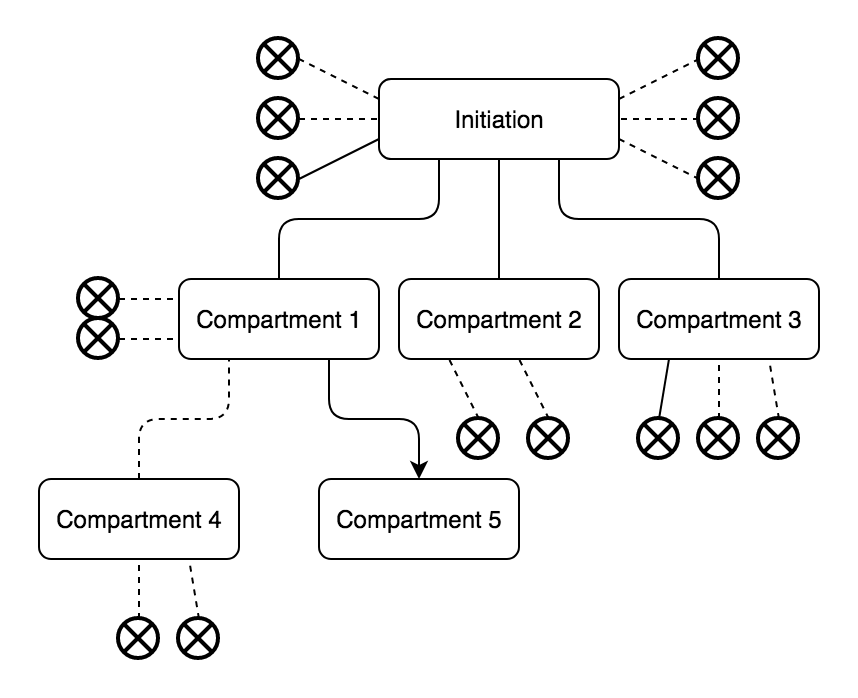
\includegraphics[width=0.5\textwidth]{Compartments}
	\caption{A graphic representation of binary compartments}
	\label{Compartments}
\end{figure}
\noindent
In Figure \ref{Compartments}, a path found by executing concolically is represented by a dashed line, while a path found by means of fuzzing is represented by a solid line. A bug is represented by $\oplus$
\subsection{Strengths}
\subsection{Weaknesses}


\section{Testing}
\subsection{Test Cases}
%Which test-cases have been used, and why?
\subsection{Results}
\subsubsection*{Comparable to non-instrumented Fuzzing}
\subsubsection*{Comparable to Symbolic Execution}

\begin{comment}

Listinglabels
diffToFuzz
SymExExample
\end{comment}

\section{Conclusion}
\subsection{Discussion}
\subsection{Future Work}
\begin{thebibliography}{9}
\bibitem{Driller}
	N. Stephens, J. Grosen, C. Salls, A. Dutcher, R. Wang, J. Corbetta, Y. Shoshitaishivili, C. Kruegel, G.  Vigna,
	Driller: Augmenting Fuzzing Through Selective Symbolic Execution,
	UC Santa Barbara,
	2016.
\bibitem{Mayhem} 
	S. K. Cha, T. Avgerinos, A. Rebert, and D. Brumley,
	Unleashing Mayhem on binary code,
	In Proceedings of the IEEE Symposium on Security and Privacy,
	2012.
\bibitem{VEX}
	N. Nethercote and J. Seward,
	Valgrind: a framework for heavyweight dynamic binary instrumentation, 
	In Proceedings of the ACM SIGPLAN Conference on Programming Language Design and Implementation (PLDI),
	Volume 42,
	pages 89–100, 
	ACM,
	2007.
\end{thebibliography}
\end{document}
